\documentclass[11pt]{article}
\newcommand{\workingDate}{\textsc{2024 $|$ Febrero $|$ 01}}
\newcommand{\userName}{Manuel Carlevaro}
\newcommand{\institution}{Visita UNAV}
\usepackage{researchdiary}

\begin{document}

\title{Diario de trabajo -- visita a UNAV}

\section*{2024.02.29}
\textbf{Tareas del día:}
\begin{enumerate}
    \item Ejecuté el programa \texttt{test-MM-K}, que usa el modelo de fricción de Karnopp, para simulaciones con 30 fases distintas $\phi$ por cada amplitud $\Gamma$, para 8 valores de $\Gamma$, con la idea de comparar con la Fig. 4 de MM. Ajusté luego cada curva con la ec. (9) de MM y obtuve el valor $\mu = 0.1095$, diferente de $\mu_d = 0.16$ que estoy usando en las simulaciones. La figura 4 que tengo para comparar estática:
        \begin{center}
            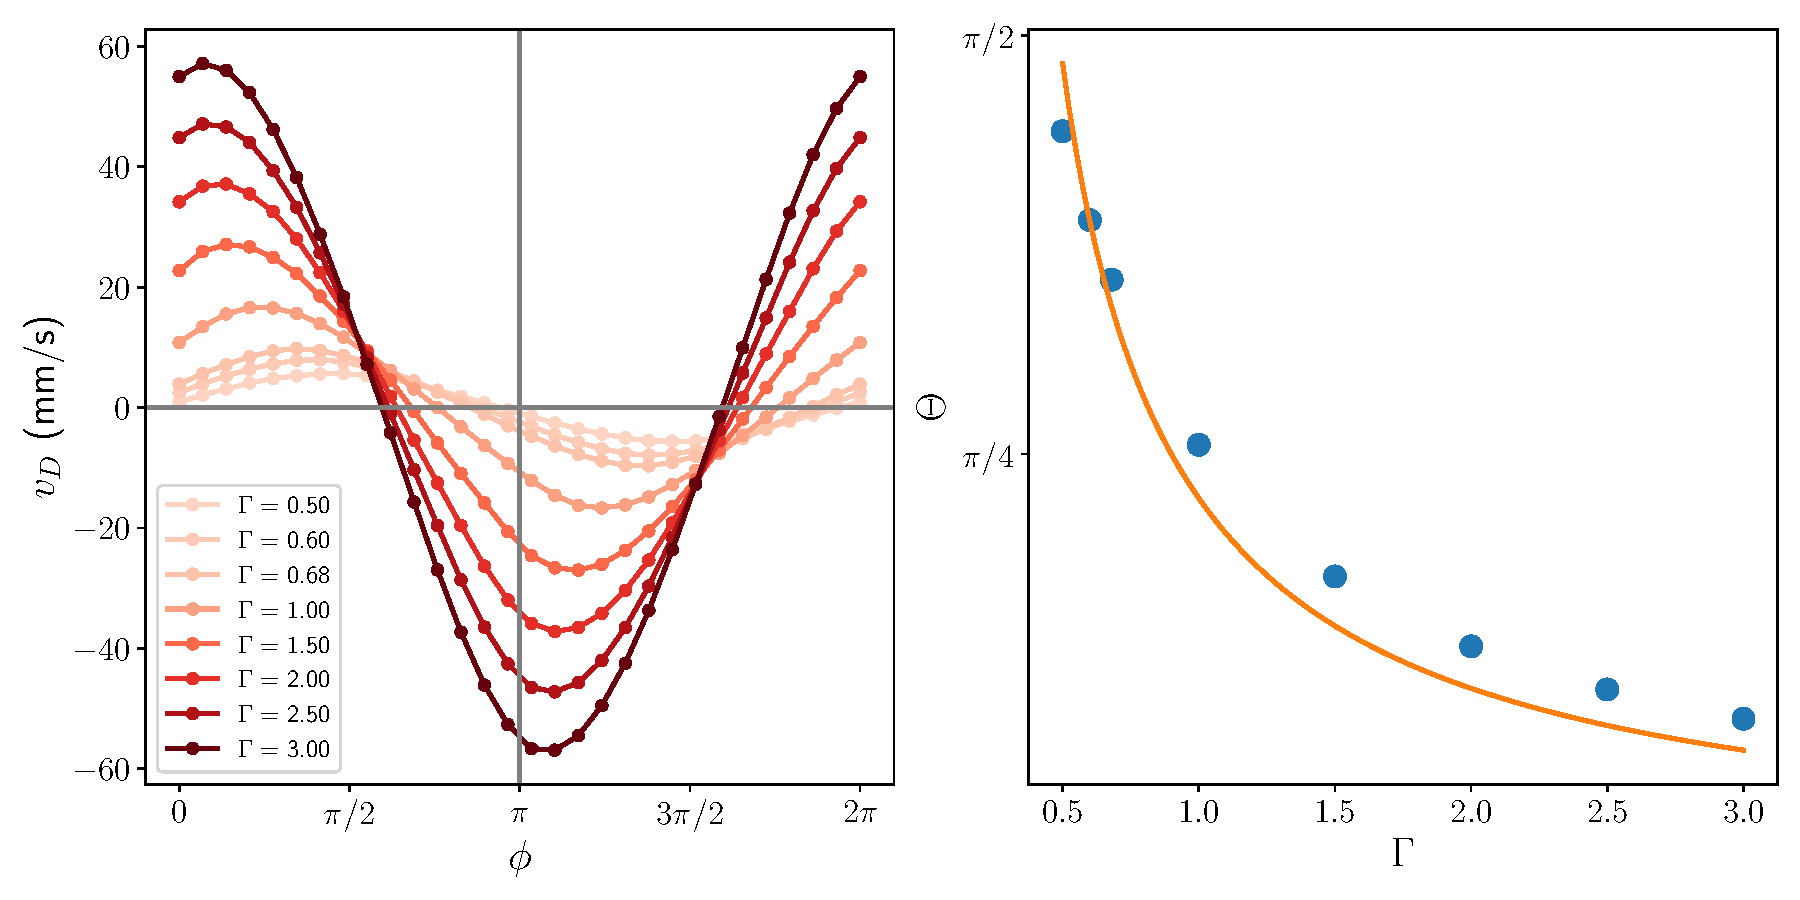
\includegraphics[width=0.8\textwidth]{figs/Fig_4_MM.pdf}
        \end{center}
\end{enumerate}


\section*{2024.02.28}
\textbf{Tareas del día:}
\begin{enumerate}
    \item Cálculo del rango de $\Gamma$: A partir de la ec. (2) del preprint MM, y usando $\rho = 1/2$, los valores de $\Gamma$ que cubren el rango de valores de $V_{\text{RMS}}$ de las curvas de la figura 2 ($(0, 100)$ \unit{mm/s}) es $\Gamma \in (0, 3.24)$.
    \item Modifico el script \texttt{set\_inis.sh} para generar los inputs con el rango anterior para $\Gamma$.
    \item Corrí dos conjuntos de 30 simulaciones con $\phi = 0$ (en \texttt{/test-04}) y $\phi = \pi/2$ (en \texttt{/test-05}). Calculé la velocidad media del móvil ajustando una recta sobre el desplazamiento (descartando los primeros valores iniciales). El resultado comparando con la Fig. 2 de MM es: 
        \begin{center}
            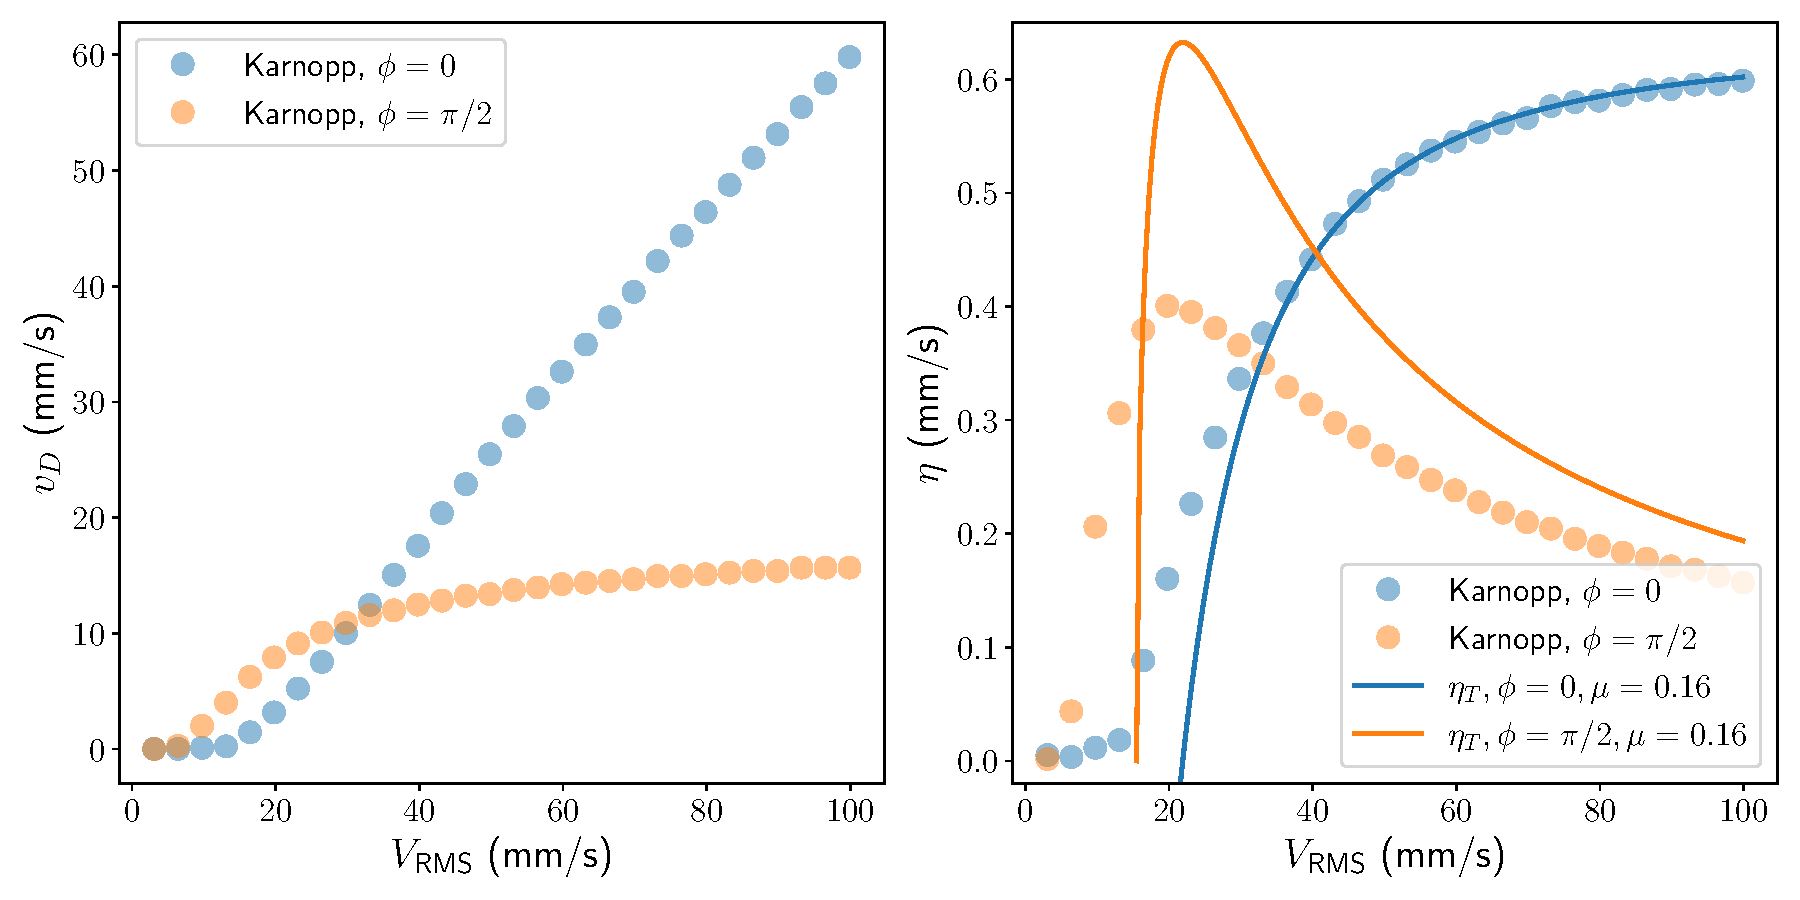
\includegraphics[width=0.8\textwidth]{figs/Fig_2_MM.pdf}
        \end{center}
        En esta figura usé $\mu = \mu_d = 0.16$.
\end{enumerate}

\section*{2024.02.22}
\textbf{Tareas del día:}
\begin{enumerate}
    \item Tomo como base el preprint MM\footnote{Efficient transport controlled by biharmonic frictional driving.} donde el input es la aceleración dada por la ecuación (1):
        \[ a_B(t) = \gamma [ \rho \sen(\omega t) + (1-\rho) \sen(2 \omega t + \phi)] \]
        En consecuencia, la velocidad y posición de la base resultan:
        \begin{align*}
            v_b(t) &= -\frac{\gamma}{\omega} \left[\rho \cos(\omega t) + \frac{(1 - \rho)}{2} \cos(2 \omega t + \phi)\right] \\
            x_b(t) &= -\frac{\gamma}{\omega^2} \left[ \rho \sen(\omega t) + \frac{(1 - \rho)}{4} \sen(2 \omega t + \phi) \right] 
        \end{align*}
        Para compatibilizar con el programa de simulación, en que el input de amplitud es la aceleración reducida $\Gamma = A \omega^2 / g$, siendo $A$ la amplitud de la oscilación en $x(t)$, escribo las ecuaciones anteriores en términos de $\Gamma = \gamma / g$:
        \begin{align*}
            x_b(t) &= -\frac{g \Gamma}{\omega^2} \left[ \rho \sen(\omega t) + \frac{(1 - \rho)}{4} \sen(2 \omega t + \phi) \right] \\
            v_b(t) &= -\frac{g \Gamma}{\omega} \left[\rho \cos(\omega t) + \frac{(1 - \rho)}{2} \cos(2 \omega t + \phi)\right] \\
            a_B(t) &= g \Gamma [ \rho \sen(\omega t) + (1-\rho) \sen(2 \omega t + \phi)] 
        \end{align*}
        También para compatibilizar con el preprint, cambio la notación en el input $\eta \mapsto \rho$.
\end{enumerate}


\section*{2024.02.13}
\textbf{Tareas del día:}
\begin{enumerate}
    \item Cambié la implementación de la excitación de la base y sumé una de dos frecuencias con la forma:
        \[ f_2(t) = \eta A \sen(\omega t) + (1 - \eta) A \sen(2 \omega t + \phi) \]
    \item Corrí el conjunto de simulaciones previo con el modelo de Karnopp, $\eta = 0.5$ y $\phi = 0.5$. Los resultados estan en \texttt{/test-03}.
    \item Se observa que la velocidad media de desplazamiento del móvil crece con $\Gamma$.
\end{enumerate}


\section*{2024.02.13}
\textbf{Tareas del día:}
\begin{enumerate}
    \item Incorporé el modelo de fricción Smooth Coulomb 2 según:
        \[ F_{sc2}(\bm{v}_{\text{rel}}) = -\mu_d m g \tanh(v_{\text{rel}} / v_d) + (\mu_s - \mu_d) \frac{v_{\text{rel}}}{v_s} \exp[-(v_{\text{rel}}/v_s)^2] \]
        donde $v_s$ es la velocidad de Stribeck. Los tres modelos tienen las gráficas (con $v_d = \qty{0.01}{m/s}$ para visualizar):
        \begin{center}
            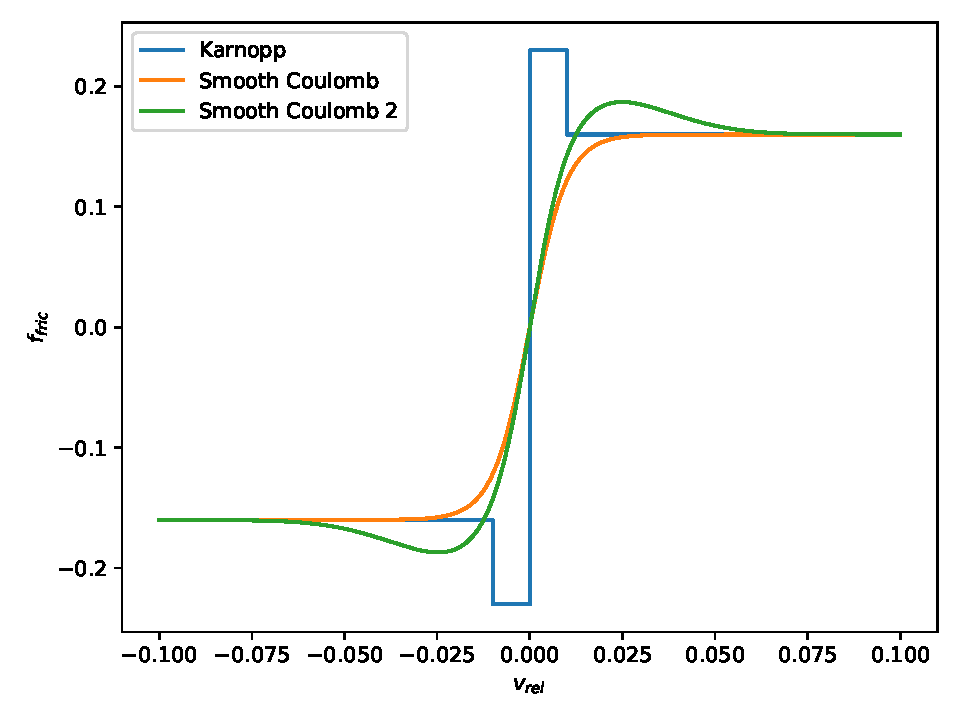
\includegraphics[width=0.5\textwidth]{figs/froce-3.pdf}
        \end{center}
    \item Corrí el conjunto de simulaciones con este nuevo modelo, y los resultados son muy similares a los anteriores, con $v_s = \qty{0.03}{m/s}$ solo para visualizar:
        \begin{center}
            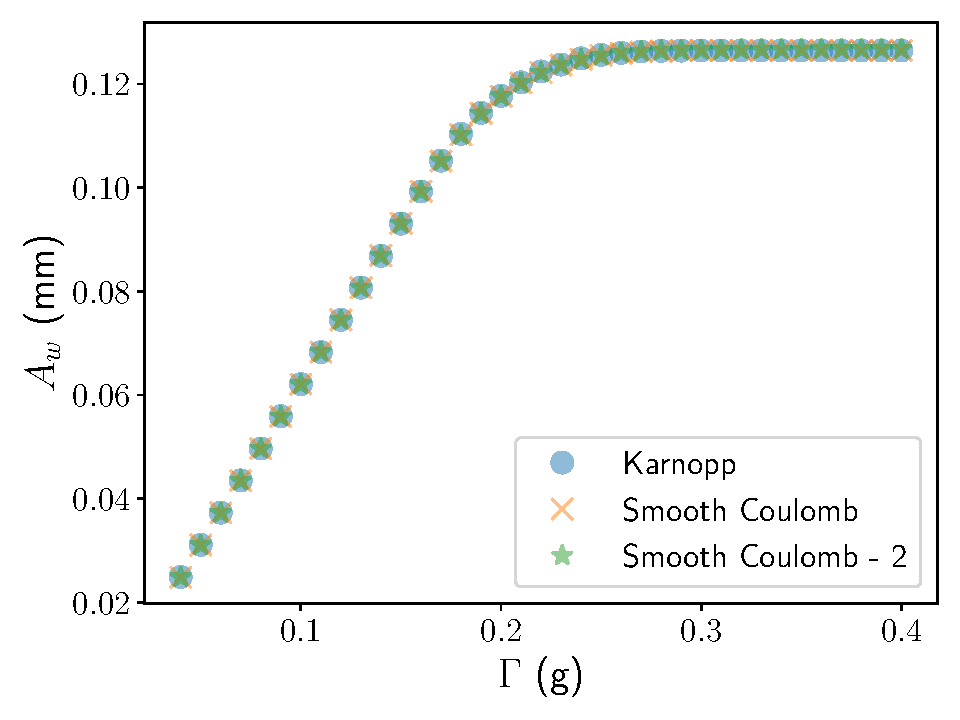
\includegraphics[width=0.45\textwidth]{figs/Fig_2_comp3.pdf} 
            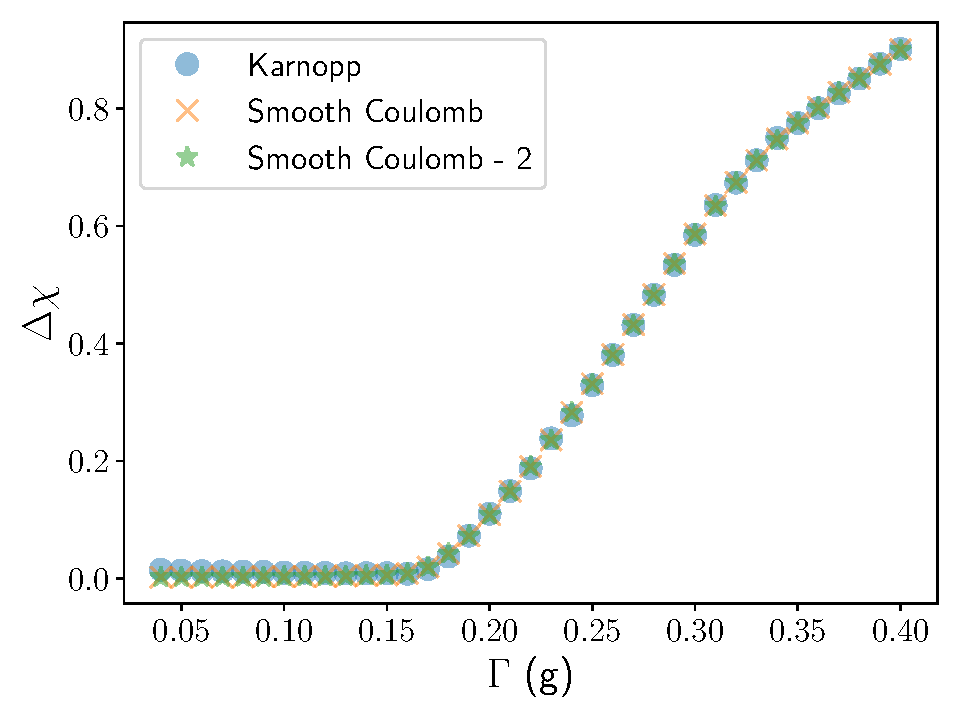
\includegraphics[width=0.45\textwidth]{figs/Fig_3_comp3.pdf} 
        \end{center}
    Los archivos están en \texttt{/test-02}.
\end{enumerate}


\section*{2024.02.09}
\textbf{Tareas del día:}
\begin{enumerate}
    \item Modifiqué los scripts para extener el rango de simulaciones hasta $\Gamma = 0.4$.
    \item Corrí de nuevo las simulaciones para los casos Karnopp (en \texttt{/test-00}) y Smooth Coulomb (en \texttt{/test-01}).
    \item Modifiqué el script \texttt{get\_amp.py} para leer el parámetro Gamma desde el archivo con los datos de salida de la simulación.
    \item Corrí los ajustes con el script \texttt{get\_amp.py} para ambos casos y rehice la Fig.2. No se observan casi diferencias entre ambos modelos de fuerzas.
        \begin{center}
            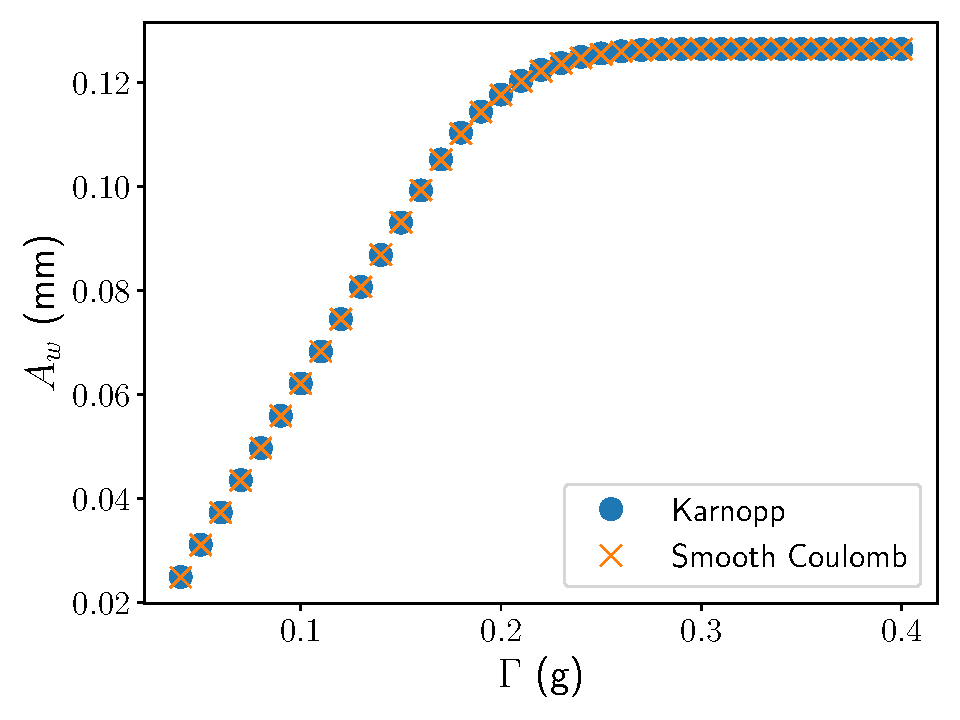
\includegraphics[scale=0.7]{figs/Fig_2_comp-1.pdf}
        \end{center}
    \item Calculé las diferencias de fase entre el movimiento del móvil y la base, para comparar con la Fig.3:
        \begin{center}
            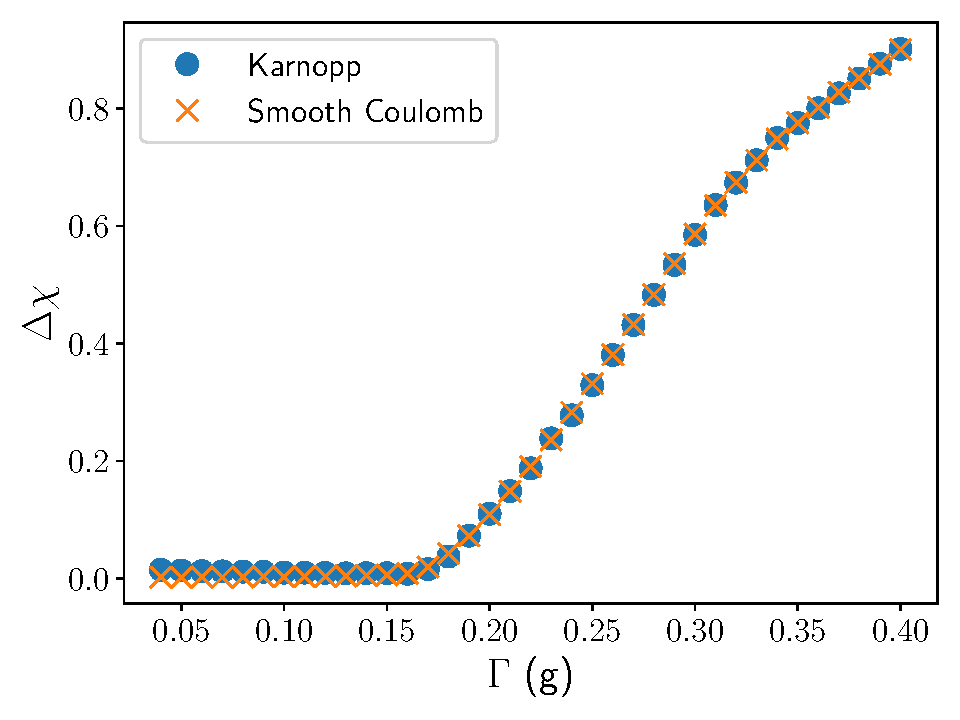
\includegraphics[scale=0.7]{figs/Fig_3_comp.pdf}
        \end{center}
\end{enumerate}
\textcolor{red}{Pendiente para el lunes:} Incoporar el modelo de fricción con exponenciales usando los valores de Diego y empezar a probar con la excitación biarmónica.


\section*{2024.02.06}
\textbf{Tareas del día:}
\begin{enumerate}
    \item Corregí un error en el código del modelo de fuerza de fricción \textit{Smooth Coulomb} según ec.(4) de Pennestri, y para $v_d = \qty{1.0e-5}{m/s}$ apareció deriva para valores grandes de $\Gamma$. Esto desaparece cuando aumento $v_d$ a \qty{1.0e-4}{m/s}. Al igual que ayer, el resultado de las simulaciones casi no se distinguen del modelo de Karnopp.
\end{enumerate}


\section*{2024.02.05}
\textbf{Tareas del día:}
\begin{enumerate}
    \item Incoporé el modelo de fuerza de fricción \textit{Smooth Coulomb} según ec.(4) de Pennestri\footcite{pennestri2016}:
        \[ F(\bm{v}_{\text{rel}}) = -\mu_d m g \tanh(v_{\text{rel}} / v_d) \hat{v}_{\text{rel}} \]
        con $v_d = v_{\text{tol}} = \qty{1.0e-5}{m/s}$.

    La salida de las simulaciones es casi indistinguible del caso con el modelo de Karnopp:
        \begin{center}
            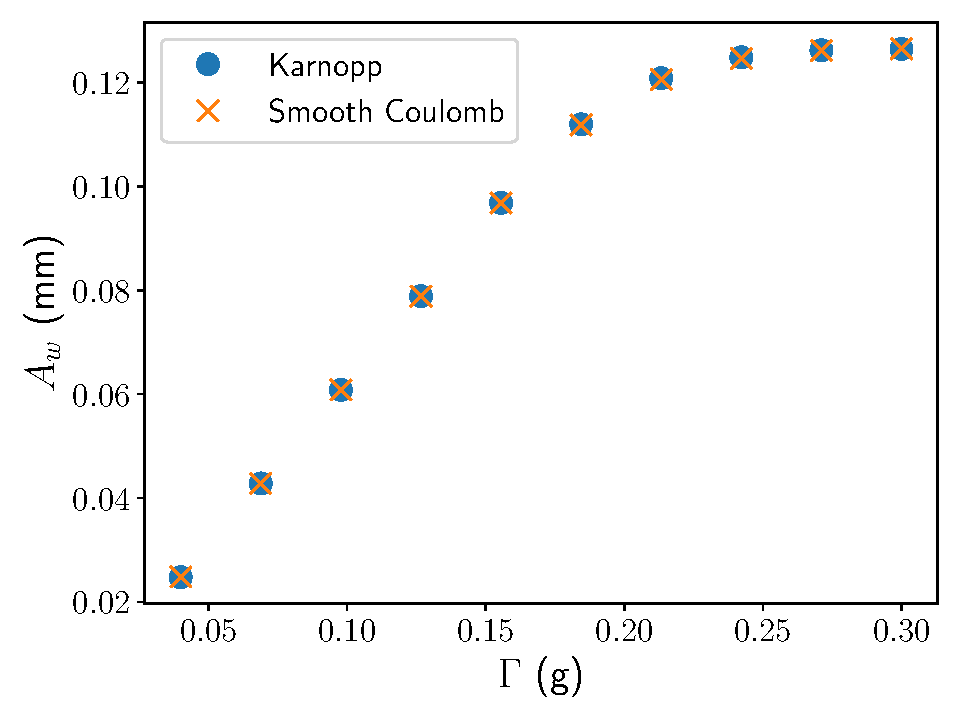
\includegraphics[width=0.7\textwidth]{figs/Fig_2_comp.pdf}
        \end{center}
\end{enumerate}


\section*{2024.02.02}

\textbf{Tareas del día}:
\begin{enumerate}
    \item Hice un script de bash para generar archivos \texttt{*.in} cambiando algún parámetro a partir de un template. El primero genera diferentes valores de amplitud de aceleración para valores de $\Gamma$ entre 0.04 y 0.3 (\texttt{set\_inis.sh}).
    \item Hice otro script para lanzar las corridas de todos los archivos \texttt{*.in} que hay en el directorio de trabajo (\texttt{run\_inis.sh}).
    \item Corregí el código para implementar el modelo de fuerza de roce de Karnopp \footcite{marques2016}, con los parámetros usados no aparece una deriva del móvil aunque si un desplazamiento inicial ($v_{\text{tol}} = \qty{1.0e-5}{m/s}$).
        \begin{center}
            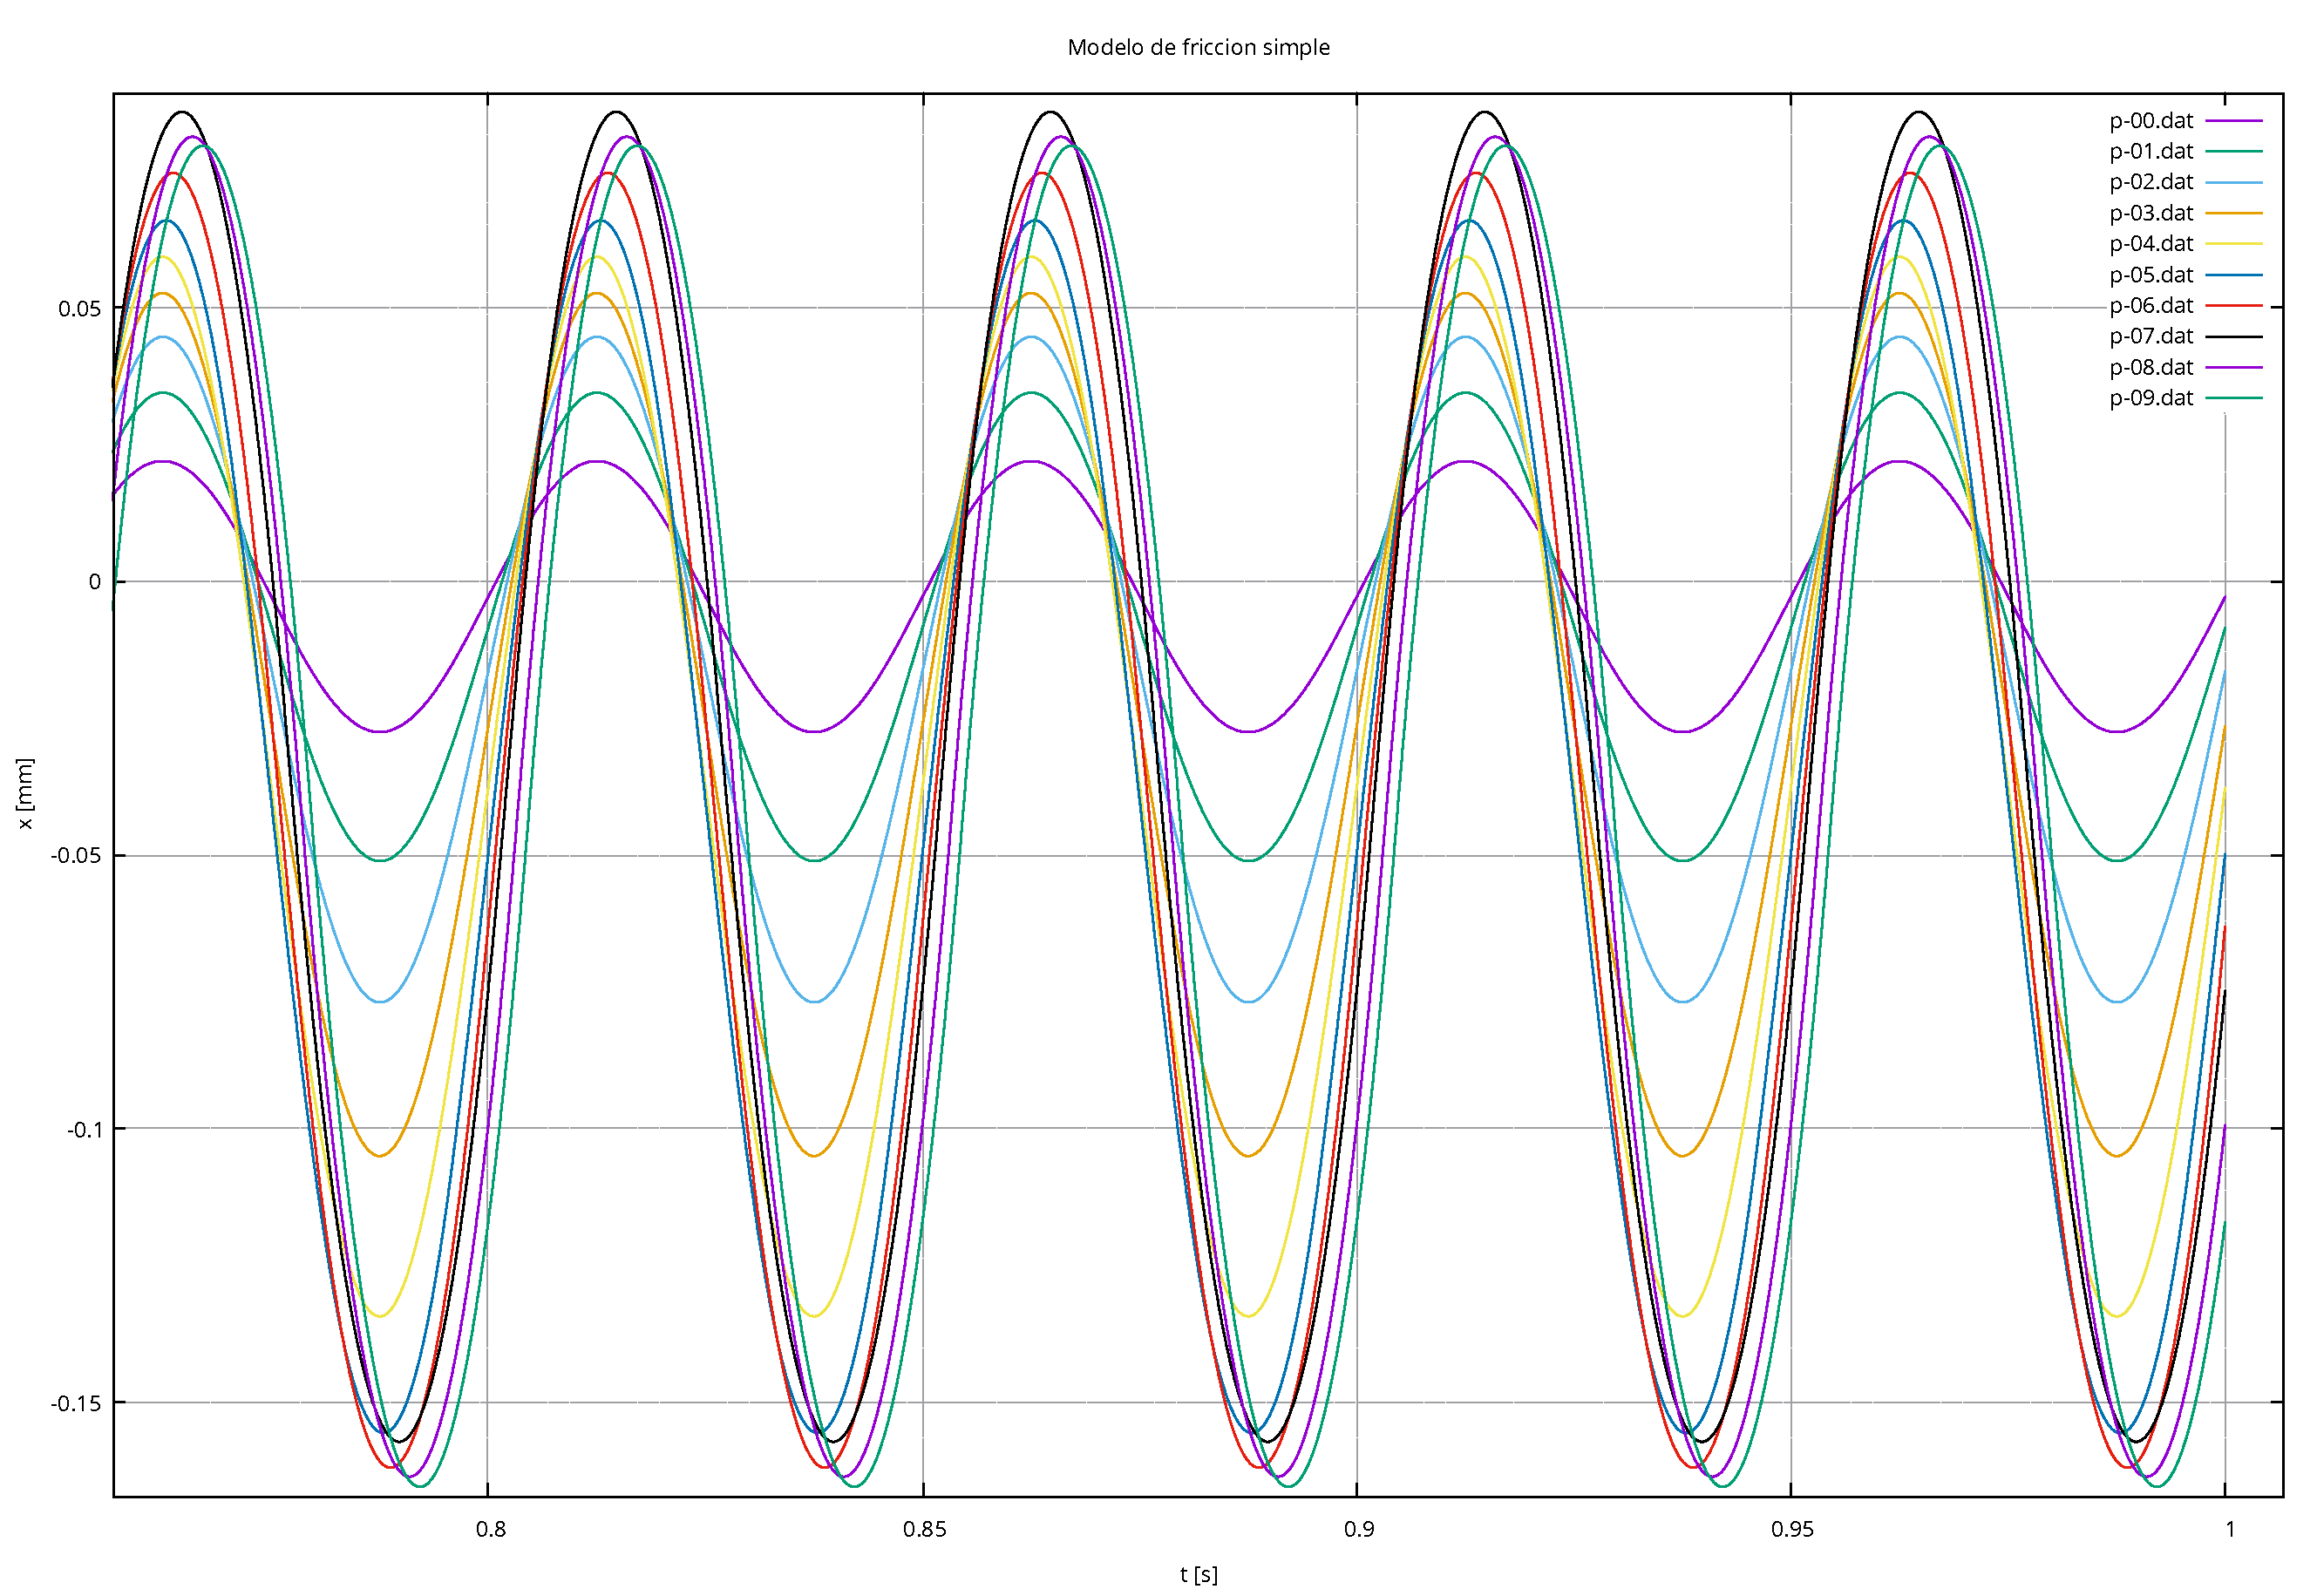
\includegraphics[width=0.7\textwidth]{figs/fig-000.pdf}
        \end{center}
        Los archivos de entrada y salida estan en el directorio \texttt{/test-00}.
\item Con las simulaciones anteriores del modelo de Karnopp grafiqué las amplitudes de los movimientos del móvil en función de $\Gamma$, dando similar a la Figura 2 del preprint Maza$^2$.
        \begin{center}
            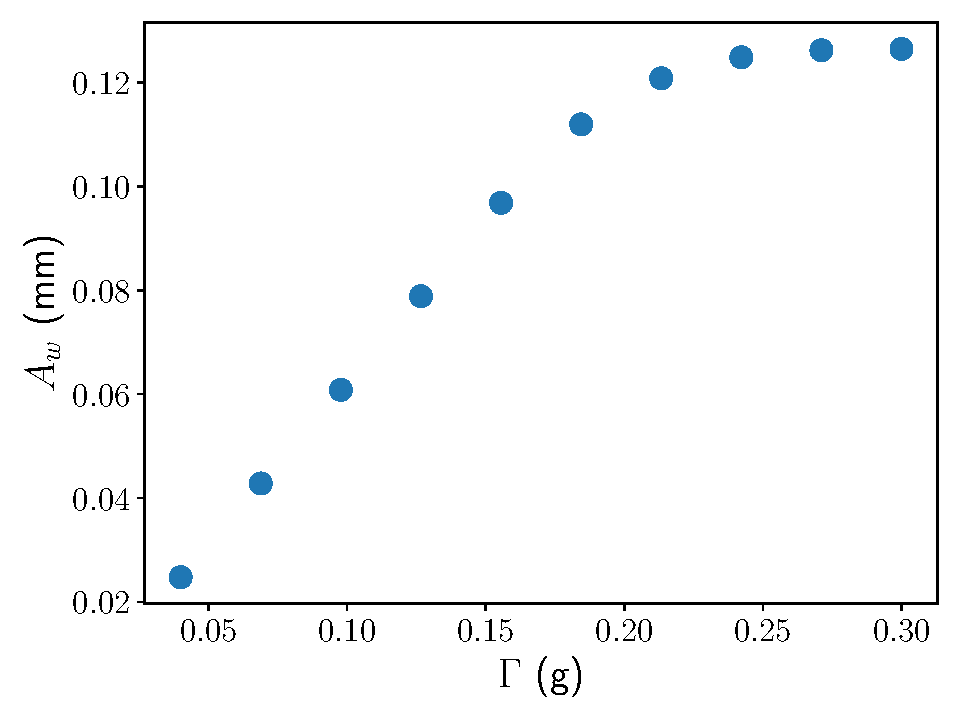
\includegraphics[width=0.7\textwidth]{figs/Fig_2_karnopp.pdf}
        \end{center}
\end{enumerate}

\textcolor{red}{Pendiente para el lunes:} incorporar otros modelos de fricción.


\section*{2024.02.01}

\section*{Parámetros para el caso de referencia}

Para comenzar como referencia uso los siguientes parámetros, a partir de los valores experimentales:

\begin{itemize}
\item Frecuencia $f = \qty{20}{Hz} \mapsto \omega = \qty{125.66}{rad/s}$.
\item Aceleración de la gravedad: $g = \qty{9.8}{m/s^2}$.
\item Aceleración reducida $\Gamma = A \omega^2/g$, donde $A$ es la amplitud de la oscilación de la base.
\item Coeficiente de fricción estática: $\mu_s = 0.2$
\item Coeficiente de fricción dinámica: $\mu_d = 0.16$
\item $\beta = \mu_d / \mu_s = 0.8$ (inicialmente).
\item El móvil es un disco de radio \qty{0.5}{m} y con una densidad de \qty{0.1021324}{kg/m^2}, lo que le da una masa $m = \qty{0.081}{kg}$.
\end{itemize}

Definiendo la velocidad relativa entre la base y el móvil como $v_{\text{rel}} = v_b - v_m$, el modelo de fricción con la base es: 
\begin{equation}
    F_f(v_{\text{rel}}) = 
    \begin{cases}
        \mu_s m g \, \sgn(v_{\text{rel}}) \txt{si} v_{\text{rel}} < v_{\text{tol}} \\
        \mu_d m g \, \sgn(v_{\text{rel}}) \txt{si} v_{\text{rel}} \geq v_{\text{tol}}  \\
    \end{cases}
\end{equation}


\textbf{Nota:} un parámetro crítico parece ser $v_{\text{tol}}$, que es el umbral por debajo del cual se activa la fricción estática. 

Tabla de amplitudes de excitación en función de $\Gamma$:
\begin{center}
    \begin{tabular}{cccc}
        \toprule
        $\Gamma$ & $a$ & $\Gamma$ & $a$ \\
        \midrule
        0.040 & 2.483e-05 & 0.184 & 1.145e-04 \\
        0.069 & 4.275e-05 & 0.213 & 1.324e-04 \\
        0.098 & 6.068e-05 & 0.242 & 1.503e-04 \\
        0.127 & 7.861e-05 & 0.271 & 1.683e-04 \\
        0.156 & 9.654e-05 & 0.300 & 1.862e-04 \\
        \bottomrule
    \end{tabular}
\end{center}
\textcolor{red}{Pendiente para mañana:} verificar el valor de $\v_{\text{tol}}$ para que no se produzca deriva en el movimiento del móvil.
\end{document}
